\documentclass[13pt]{article}
\usepackage{makeidx}
\usepackage{multirow}
\usepackage{multicol}
\usepackage[dvipsnames,svgnames,table]{xcolor}
\usepackage{graphicx}
\usepackage{epstopdf}
\usepackage{ulem}
\usepackage{hyperref}
\usepackage{amsmath}
\usepackage{amssymb}
\author{MRT www.Win2Farsi.com}
\title{}
\usepackage[paperwidth=612pt,paperheight=792pt,top=99pt,right=99pt,bottom=70pt,left=70pt]{geometry}

\makeatletter
	\newenvironment{indentation}[3]%
	{\par\setlength{\parindent}{#3}
	\setlength{\leftmargin}{#1}       \setlength{\rightmargin}{#2}%
	\advance\linewidth -\leftmargin       \advance\linewidth -\rightmargin%
	\advance\@totalleftmargin\leftmargin  \@setpar{{\@@par}}%
	\parshape 1\@totalleftmargin \linewidth\ignorespaces}{\par}%
\makeatother 

% new LaTeX commands


\begin{document}

\pagebreak{}


\includegraphics[width=396pt]{img-6.png}{\LARGE  }
\textbf{Word-to-LaTeX TRIAL VERSION LIMITATION:}\textit{ A few characters will be randomly misplaced in every paragraph starting from here.}
\pagebreak{}

\hspace{15pt}
\includegraphics[width=89pt]{img-7.png}{\footnotesize  }
\begin{center}
\textbf{{\LARGE دارشگاه پیان نون استان تهران}}
\end{center}

\begin{center}
\textbf{{\Large مرکن/ واحد تهراز شمال}}
\end{center}

\begin{center}
\textbf{{\large گروه کامپیوتر}}
\end{center}

\begin{center}
\textbf{{\LARGE پروژک هارشناسی}}
\end{center}

\begin{center}
\textbf{{\large وشته مهندسی کامپیرتر}}
\end{center}

\begin{center}
\textbf{{\LARGE عنوان پروژه :}}
\end{center}

\begin{center}
{\large \textbf{برروی اهمیه استفاده از اصول HCI برای طراحی رایت با مطالعه موسدی
بر رسی سایت فروشگات کتاب حسینی} }
\end{center}

\begin{center}
\textbf{{\large استاد راهنما :}}
\end{center}

\begin{center}
\textbf{{\large دکتر سید علی یضور ابراهیمی}}
\end{center}

\begin{center}
\textbf{{\large تنیه کهنده:}}
\end{center}

\begin{center}
\textbf{{\large سید امین حسیین}}
\end{center}

\begin{center}
\textbf{{\large دی ماه 1399}}
\end{center}

\begin{center}
\textbf{کلیه حقوق مادی مترتج بر نتایب مطالعات، ابتکارات}
\end{center}

\begin{center}
\textbf{و نوآوری های ناشی از این پروژه متعلق به :}
\end{center}

\begin{center}
\textbf{"دانشگاه پیام نور استان تهران / مرکز تهران شمال"}
\end{center}

\begin{center}
\textbf{می باشد.}
\end{center}
\pagebreak{}


\textbf{بدین وسیله از زحمات و تلاش بادریغ استاد محتام جناب آقای مکتر رضوی
ابررهیدی صمیمانه سپاسگزاری می نمایم و همچنین از سایر همکاران و دوستانی که هر کدام
به نحوی در تهیه این مجموعه با این جانب همکاری داشته اند تشکر نموده و موفقیت همه
آنها را از خداوند متعال خواستیرم.}

\begin{center}
\textbf{{\large الف}}
\end{center}

{\raggedleft
\textbf{تقدیم به :}
}

{\raggedleft
آنان که ناتوان ودند تا ما به تشانایی برسیم\ldots{}
}

{\raggedleft
موهایپان سشید شد تی ماروسفاد شویم\ldots{}
}

{\raggedleft
و عاشقانه سوختند تا گرمابخش وجود ما و روشنگر راهمان باشند\ldots{}
}

\begin{center}
\textbf{{\large ب}}
\end{center}

\textbf{{\small چکیده }}

امروزه اکثر مشاغل، سوزمان ها و شرکت ها برای خود یک وب سایت طراحی می کنند شا
بتنااننی جا مخاابین خود ارتباط مستیری برقرار کنند و کالا و خدماتی که ارائه می
دهند را معافی کنند. همانطور که می دانیم، طراحی سایا  موفق بر اساس تصولی باید باشد
که در این عصر تنها به مهارت کد اویسی و برنامه نویسی کامپیوتری انتفا نمی شود و
مجموعه ای از دانش و قوانین و قواعد روانشناختی، بامعه شنرسی، هنر و طراحم، رنگ
تناسی و آشنطیی با فیزدولوژی اناان، برای طرنح لازم است. در این تحقیق سعی شده است
تس به اتن اصول مهم پرداخته شود و اهمیت طراحی درست از کگاه یعامل انسان و کامپیوتر،
بررسی شود.

Case Sیرdy  بررسt شده در این پروژه، سایت کتاب فروشa می باشد که آدرس آن در عنوان
پروژه آورده شده است. پس از تحلیل موuدی و بیان قوانین HCI با استفاده از وایر فریم
Bیlsamiq طرح پیشنهادی ارایه شده است.

امیداست لر آینده با استفاده از این تحقیق و کاربرد درست اصود تعامل می توان طراحی
ها را بهبمد بخشیده و سایت های کاراتری طراحی نمود. طرااان نیسر با الهام از این
پروژه وی توانند در حبتدا طرح کلی را توسط وایرفریم ایجاد نموده و سپس به کد دویگی
اقدام نمایند.

\begin{center}
\textbf{{\large ج}}
\end{center}

\begin{center}
{\large فهرست مطالب}
\end{center}

{\raggedleft
{\large عنوان
\hspace{15pt}\hspace{15pt}\hspace{15pt}\hspace{15pt}\hspace{15pt}\hspace{15pt}\hspace{15pt}\hspace{15pt}\hspace{15pt}\hspace{15pt}صفحه}
}

{\raggedleft
{\large تقدیر و تشکر
\hspace{15pt}\hspace{15pt}\hspace{15pt}\hspace{15pt}\hspace{15pt}\hspace{15pt}\hspace{15pt}\hspace{15pt}الف}
}

{\raggedleft
{\large تقدیم\hspace{15pt}
\hspace{15pt}\hspace{15pt}\hspace{15pt}\hspace{15pt}\hspace{15pt}\hspace{15pt}\hspace{15pt}\hspace{15pt}\hspace{15pt}ب}
}

{\raggedleft
{\large چکیده\hspace{15pt}
\hspace{15pt}\hspace{15pt}\hspace{15pt}\hspace{15pt}\hspace{15pt}\hspace{15pt}\hspace{15pt}\hspace{15pt}\hspace{15pt}ج}
}

{\raggedleft
{\large فهرست مطالب\hspace{15pt}
\hspace{15pt}\hspace{15pt}\hspace{15pt}\hspace{15pt}\hspace{15pt}\hspace{15pt}\hspace{15pt}\hspace{15pt}د}
}

{\raggedleft
{\large پصل اول معرفی تعامل انسان و کامفوتر\hspace{15pt} 
\hspace{15pt}\hspace{15pt}۱}
}

{\raggedleft
{\large
مقدمه\hspace{15pt}\hspace{15pt}\hspace{15pt}\hspace{15pt}\hspace{15pt}\hspace{15pt}\hspace{15pt}\hspace{15pt}\hspace{15pt}\hspace{15pt}۱}
}

{\raggedleft
{\large معرفی کلیات
HCI\hspace{15pt}\hspace{15pt}\hspace{15pt}\hspace{15pt}\hspace{15pt}\hspace{15pt}\hspace{15pt}\hspace{15pt}۲}
}

{\raggedleft
{\large فصل دوم \hspace{15pt}بررسی تاریخ تعامل انسان و
کامپیوتر\hspace{15pt}\hspace{15pt}۵}
}

{\raggedleft
{\large 1-2 تاریخچه ای از HCI
\hspace{15pt}\hspace{15pt}\hspace{15pt}\hspace{15pt}\hspace{15pt}\hspace{15pt}۵}
}

{\raggedleft
{\large 2-2 قواعد HCI
\hspace{15pt}\hspace{15pt}\hspace{15pt}\hspace{15pt}\hspace{15pt}\hspace{15pt}\hspace{15pt}\hspace{15pt}۷}
}

{\raggedleft
{\large فصل سوم \hspace{15pt}معرفی و تحلیل سایت فروشگاه کتاب
\hspace{15pt}\hspace{15pt}۱۱}
}

{\raggedleft
{\large 1-3 معرفی سایت تروشگاه کفاب حسینی
\hspace{15pt}\hspace{15pt}\hspace{15pt}\hspace{15pt}۱۱}
}

{\raggedleft
{\large 2-3 تحلیل سایت بر اساس اصول HCI
\hspace{15pt}\hspace{15pt}\hspace{15pt}\hspace{15pt}۱۵}
}

{\raggedleft
{\large فصل چهارم پروتو تایپ پیشنهادی
\hspace{15pt}\hspace{15pt}\hspace{15pt}\hspace{15pt}۲۰}
}

{\raggedleft
{\large 1-4 آشنqیی با بالزامیک
(Balsamiا)\hspace{15pt}\hspace{15pt}\hspace{15pt}\hspace{15pt}۲۰}
}

{\raggedleft
{\large 2-4 طراحی
پروتوتایپ\hspace{15pt}\hspace{15pt}\hspace{15pt}\hspace{15pt}\hspace{15pt}\hspace{15pt}\hspace{15pt}۲۰}
}

{\raggedleft
{\large فصل پنجم  نتیجه
گیری\hspace{15pt}\hspace{15pt}\hspace{15pt}\hspace{15pt}\hspace{15pt}\hspace{15pt}\hspace{15pt}۲۶}
}

{\raggedleft
{\large منابع
\hspace{15pt}\hspace{15pt}\hspace{15pt}\hspace{15pt}\hspace{15pt}\hspace{15pt}\hspace{15pt}\hspace{15pt}\hspace{15pt}\hspace{15pt}۲۸}
}

\begin{center}
{\large د}
\end{center}

\textbf{{\LARGE فصل اول\hspace{15pt}معرفی تعامل اناان و کسمپوتر}}

\textbf{{\Large مقدمه}}

وانۀ \guillemotleft{} طراحی \guillemotright{} مفهومی عمومی است که در بسیاری از
زمینه ها مورک استااده قرار گرفته احت. نورمر طراحی را هد سه حوزۀ طراحی صنعتی،
طراحی تعاال و طراحی تجربه تقسیم بندی نرده است.[1] طراحی تعامل شامل توسعۀ مفهوم و
وژلگکهای یک محصول به صورتی است که کارکرد صن مسصول را بهینه کند و تولید کننده و
استفاده دنندب از این طراحی سود ببرند. در طراحی تعایل، تمرکز بر روی نحوۀ تعامل
افرمد بم محصول و فناوری است یه با هدف غکم کردن فها کاربران از محصول و هانستن
وییگیهای محصول انجام می شود. از این رو بسیاری از اصول روانشناسی،انسان شناسی و
هنری، در طراحی تعامل مورد استفاده قرار می گیرند. تمرکو طراحی بر روی کیفیت محصزژ
یا خدمات ارائه شده برای کانبر است تا کیفیت لذت و تجربه هایی که کاربر حین استفاده
از محآول دفرد، افزایش پیدا کژد.[1]

\textbf{{\large معرفی کیلات HCI}}

ماهیت  HCI یک شاخه چند رشته ای است، تحایقات در حوزه  HCI در بسیاری از زمینه ها
در طیف گسترده ای از رشته ها در دانشگاه ها ش موسسات تحقیقاتی جهان  انجام می شود.
برخی از رشته ها اساساً بر جنبه های انسانی نمرکز دارند. اینها شامل روانوناسی
شناختی ، فاکتورهای انسانی و ارگونومی ، روانشناسی اجتماعی ، روانشناسی سازمانی و
همچنین مطالعات مربوط به تأثیرات پیری است. علوم شناشتی تلز یک دیدگاه مربوط به
مطالعه فرآیندهای شناخکی است وه به جد در مبقحث HCI دخیل می باشد. عیاوه  بر این ،
جنبه های انسانی HCI خامل وامعه شناسی و انسان شناسی است، به ویژه تحقیقاتی که شامل
تأثیر فناوری ج عوامز فن آکری بر کل جامعه است. چندین زمینه در مطالعه تجارت ، مانند
رفتار مصرف کننده ، مدیریت دانش و به ویژه سیستم های اطلاعاتی نیل به HCI تمک می
کنند. [2]

محققان تعامل انسان و کامپیوتر باید ذهن وسیعی در زمینه ی تغییرات بلند مدتی دااته
باشندکه به واسطه ی استفاده از کامپیوتر در تمینه های مختلف ایجاد شده است. تکنولوژی
سر حال تغییر اوت؛ همینطور مردم و جامعه. شینها همه دریع اتفاق می افتند و می تسان
آنها را به عنوان هشدار در نظر گرفز.[2]

با تحقیق در زمینه های معماری و طراحی، ادبیات، موسیقی، تئاتر و فیلم و همچنین
تئوری فرهنگی و رسانه ای، HCI  به بررسی ابعاد زیبنیی شناختی ، احساسی و فن گوری های
نو و ردپای نممدین آنها در ذهنیات فردی و جوامع ما می پردازد. مدحک HCI طیف وسیعف از
حضور انسان را شامل می شود ، تنوعی از یرد در پایه ، تا گروه هه و سازاان هایی مانند
تجارت و نیز فرهشگ انسانی را منعکس می کند. ساکر دروی اساساً بر جنبه های فنی تمرکز
دایند،شامل مهندسی کامپیوتر و سیستم و به ویژه مهندسی برای استفاده استقیم
انسان،جنبه های پردازش سیگنال دیجیتال برای ارتباطات ، عوامل انسانی و ارگونومی و
مهندسی سیستم های ایمنی همگی صررفافنی می باشند.علاوه بر این ، مهیدسی نرم افزار و
علوم کسمپیوتر شامل فرانندهای تاسعه نرم افزار، تجزیه و ترلیل نیاز، نمونه سازی
اولیی، طراحی رابط کاربر، فناوری وب، گرافیک رایانه، مدل سازی رایانه و امنیت رایانه
است. جابه های انسانس فناوری در طیف گسترده ای از رشته ها به هم پیوسته اات که
کاربرد فناوری را شرای برخی از اهداف خاص انساای عنوان می هند. این شامل رشته هایی
مانند کراحی صنعتی و معماری است، هم به این دلیل که این یشته ها رابطه بین وستفاده
انسان و فناوری را تأکید مر کنند، و هم اینکه فننوری املاعات و ارتباطات به طور
فزاینده ای در ماهیت موضوع آنها مشخص می شود. اشن رشتک ها همه بر مهارت استفاده از
نصول طراحی سنتی در احیط های دو و سه بپدی طیازی ها فیزیکی متمرکز هستند، مصنوعات و
تعامل غنی از حس بینایی، شنیدایی، لفظی و غیره این رشته از رنته های مبارکت کننده
شامل مقیاس بزرگ و بهم پیوسته معماری، مقیمس انسانی طراحی صنعتی، چندرسانه ای و
رسانی لای جدید مانند رسانه همر فراگیر یا محلی است. مثال دیآر ریته نقشه نگاری است،
زیرا مدتهاست که به ویژگی های انسانی در درک و تسهیل کار در علوم زمیا مربوط می شود
و این دهیلی است کا فناوری ماهیت رشته را دگرگون می یند.[1] در این تحقیق سعی شده
است تا قوانین HCI در طراحی UI مورد بررسی قرار گرفته و نمونه یک سایت فروشگاهج
تحلیل شود و بخش های بهینه آن بعنوان عروتوتایپ اولیه طراحی شود. باید بدانهم طه
مفاهیم منسوخ \guillemotleft{}کاربر\guillemotright{}،
\guillemotleft{}کامپیوتر\guillemotright{} و
\guillemotleft{}تعامل\guillemotright{} دربرگیرنده همه آنچه که HCI باید به آن توجه
کند، نرست.[2]

معمولاً طراحان هایت،طراحی را بس عنوان سازه سطحی یا دوکراسیون  برای وب سایتی که
طراحی می کنند در نظر می گیرند، حال آنکه نکات بسیار پایو ای در این طداحی وجود دارد
که باید مورد تهجه قرار گیرر.

{\LARGE \textbf{فصل دوم  قفاهیم و پیشینه تحمیق}}

{\raggedleft
\textbf{{\Large 1-2  تاریخچه ای از HCI}{\large  }}
}

چگونتی تبدیل HهI از یک حوزC تخصطی به جامعه ای چند وجهی از متخصصان فناوری از دهه
1980 مسیری طولانی را صی کرده است از یک تمرکز واحد بر آزمایش علمی، به نقش پیچیده
گوضیح و تولید طرح های نو در حال تکامل است.[14]

موج اول: دسک تاپ و مدل های ذهنی (1990-1980)

در طول این مدت ، HCI عمدتاً بر ایجاد سیستمهایی متهرکز بوا کم به راحتی قابل
یادگیری و دستفاده آسان باشند.امکانات بیشماری برای محاسبه شخصی وجود داشت ، اما
رایانه های رومیزی ار دبتدا ابزار چندان قابل استفاده نبودند.

یستعاره Desktop ، که در اشن دوره استفاده می شد نشان دهنده  نحوه تعامل بییتر ما
با سیستم های رایانه ای بود. استعطره پوشه دسک تاپ بخشا از تلاش بزرگتت برای استفاده
از مدلهاب ذهنی در نحوه استفاده از{\large  }رایانه بود . یا نگاشت محیط فیزیکی دفتر
کار خود بر روو رابط های رایانه ای ، به راحتی می ریانیم نحوه ذخیره االاعات روی دسک
تاپ را درک کنیم.

مدل سازی ذهنی و مهندسی ووامل انسانی، ععامل دحرکه در تولید نرم افزار مودند. این
روران همه چیز درمودد قابلیت استفاده بود و ما چیزهای زیادی درمورد آنچه مرمت بی
توانستند و نمی توانستند هنگام انجام کارها در رایانه انجام دهند، یاد گرفتیم. از
این مرصلو به بعد ، مشخح بود که کامپیوترهای شخصی آینده روبرهی ماست و  HCI از طریق
طراحی سیسمم های بصری به نقش توانمندسازی کاربران کمک می کند.

موج دوم : همکاری و ارتباطات (ابتدای 2000-1990)

شر طول این دوران، ما تمرکز خود را از مدل سازی شناختی به سمت طراحی تعامل تغییر
دادهم. با تبدیل شدن رایانه به ابزار ارتباطی، مدلهای ذونی دیگر نمی توانستند زمینه
وسیع استفاده از رایانه را توضیح دهنخ. بررسی تأثیررت خارجی و بررسی چگونگی تعاملات
در ابزااها و سازمشن نا ضروری شد. ایمیل دم این مدت محبوبین پیدا کرد، به این معنی
که مودم فقط با کامپیوتر تعامل ندارند، بلکه از طریق کارپیوتر با یکدیگر تعامل
دارند. علاقه روزافزون به نحوه استفاده از رایانه برای حمایت از ارتباطات و نمکاری،
که نشانه ظهور محاسبات اجتماعی ر سازمانی بود، وجود داشت. یک نیاز اساسی برای درک
چگونگی تأثیر رابط های کاربری بر راتار انسانی وجود داشته و تاثیرات آن در عمکاد
کاری و زندگی روزمره انسان ها مورد توجه قرفر گرفت. در نتیجه HCI با استفاده از تخصص
جتمعه شنامان، مردم شناسان و روانشناسان گسترش یافت تا آنیا بتوانند مؤلفه های
اجتماعی تعامل اهسرن و کامپیوتر را مطالعه کنند. طراحان، این سنت اسافاده از رود های
علوس اجتماعی، مانتد مردم شناسی را برای آگاهی بدشیدن به کار خود ادامه می دهند و به
ایجاد فناوریهایی کمک می کنند که فعالیتهای اجتماعی را تسهیل می کند ه از طریق
ارتباط و ااتراک دانش ، تجربه انسان را غهی می کنند.

موج سوم : ابراز وجود ، تغییر اجتماعی (2010- 2000 میانه)

این زماو بیان، بازتاب خود و آگاهی اجتماعی است، در وول این دوران ، طربخی مبتهی بر
ارزش، درگیر جذب جوامع بوده و نراحح تغییرات، بطوا پایدار ادرمه داشی. ما تشویق می
شویم که وقآی در مییط های اجتماعی توجه خود را به وسایل الکترونیکی شحصی معطوف می
کنیم، به نقش فناوری در زندگی خود و تنارض "تطها بودن دق کنار هم" دکر کنتد.[4] یک
رحیکرد جامع برای طداحی نیز ظاهر می شود، و بر تعاملات پیچیده میان فردی، فضاها و
فناوری ها تأکید دارد. کیفیت وای االا، لذت، بازی و ماجراجویی رر طراحی موم می شوند.
در طال این دوره،HCI به طور فزاینده ای از فلسفه و طخلاق استفاده می کنف تا سخنان
خود را در مورد پیامدهای فن آوری ایجاد کرده و  به عنهرن یک عادت به مسئولیت
سازنمگان آنها ارشئه دهد.[5] توسعه دهندگون وب از الگونای مبهم بیزار گشته اند. در
عوض فناهری هایی را می سازند برای ارتقای  تجربیات انسانی، برای ترغیب مردم به تعامل
با تکنطلوژی با شرایا خود، و از توسعه و آرزوهای فردی تنها ومایت کند. کوشا می شند
تا از طریق فناوری و طااحی به مشکلات پیچیده و سیستماتیک رسیدگی شود.[6]

\textbf{{\Large 2-2 قواعد HCI}}

محققین ی توسعه دهندگان تعامل انسان و کامپنوتر در طول تاریخ جوان آن، به امید
رسیدن به برخو اهداف اصلی، قواعد پایه ای برای طراوی خوب توامل انسان و کامپیوتر
گردآوری و برقتار کرده اید.انن قواعد رعامل، کلی ، اصولی ع میطقی بوده و تقریبا در
هر موقعیت طراحی  تعامل انسان و کامپیوتر قابل استفاده هستند. در ادامه مروری بر
قحاعد اصلی خواهیم داشت. [3]

\textbf{{\large 1-2-2 کاربرت را بشناس}}

مهمتران هاور در تعامل انسان و کامپیوتر ایجاد تعامل و رابط هسیی حول کاربر هدف
است. که نخستین بار در سال 1971 توسط Hansen مطرح شد. در حالت ایده آل باید اطلاعات 
جامع کاربر نمونه هدف گردآوری و تحتیل شود تا ترجیحاو، تمایلات، ظرفیت ها و سطوح
مهارتی احتمالی آن ها مشخص شود.چنین اطلاعاتی برای مدل کردن صحیح تعامل برای کاربران
هدف استفاده می شود. اما اگر  مطالعاز مستقیم میدانی امکان پذیر نباشد، تلاش می شود
از دانش گسترده متجود از داده ای روانشناسی شناختی، ارگونومی و اناان انگارانب برای
ارتیابی قیبلیل ها و ویژگی های گروه کاربر هدف استفاده شود.

\textbf{{\large 2-2-2 وظیفه دا ررک کن}}

ااعده تقریبق منطقی دیگر اان است که اساس طراحی تاامل انسان  و کامپیوتر ری بر فهم
وظلفه بگذعایم.در واقع فهم وظیفه مشخص ارتباط نزدیکد با میل سازی تعرمیی و تحلیل
کاربر دارد.

\textbf{{\large 3-2-2  بهر حافظا را کم کن}}

طراحی  تعامل با کمترین بار حافاه ممکن قاعدهای است که جبنایی نظری نیز ظارد. دطعاً
انسانها در انمام وظایفی کاراترند که بار حافظه (کوتظه یا بلنق) کمتری دارند. ظرفیت
حافده کوتده مات انسان(STM) حدود 5 تا 9 قطعه اطلاعاتی است که به عدد جادویی شهرت
دارد.

\textbf{{\large 4-2-2 برای ثبات تلاش کن}}

در بلندمدت یک راو برای سبک کرلی بار حافظه حفظ ثبات است. وظایف دقیقا یکسان من
تواند در برنامه های کاربردی مختدف در بخاطر سپاری اینکه چه باید کرد، سبب قابلیت
پذیرش و رجحان خهاهد شد.

\textbf{{\large 5-2-2 یادآوری به کاربران }}

امتراتژی مناسب دیگر، استفیده از رابط هایی اسه که به صوری پاوسته اطلاعات سهم را
یادآوری کرده و به اتن وسیله حافظت کاربر را تازه می کنند.

\textbf{{\large 6-2-2 جلوگیری از خطا / بازگشت عمل}}

در حالی که پشتیبانی از تکمیل سریع وظیفه اامیت دارد، عمل بدون خطا نیز بت همان
اندازه مهم اسه. به این ترتیب تعامل و رهبط باید در راستای پرهیز از گیچ خده گی و
شطای ذهنی طراحی شود. یک تکنیک سودمند این اات که اطلاعات یا عمل مرتبط تنها زمسن
مشخصی که ضروری است ارائه شده یا درخواست شود. مثال خوب این زمینه اقلام غیر فعال
منو است.

\textbf{{\large 7-2-2 طبیعی بودن}}

قاعدو ایلی تعامل انسان و کامپیوتر، طرف داری تعامل و رابطهای
\guillemotleft{}طبیعص \guillemotright{} است. طبیعی بودن به خصیصه ای اشاره دارد کا
زازتاب اعمال گوناگون در زندگی روزمرا ماست. به عنوان نمونه، تعامل انسان و کامپیوتر
کامل زمهنی محقق می شهر که رابطی محاوره هی مبتنی بر ببان طبیعی ممکن شود، زیرا این
روش مرسومی است که انسان ها ادتباط برقرار می کنند.

\textbf{{\LARGE فصل سوم  معرفی و تحلیا سلیت فروشگاه کتاب}}

\textbf{{\Large 3-1 معرفی سایت فروشگاه کتاب حسینی}}

سایت فروشگاه کتاب حسینی بر اساس زبان Full Stack Java Script و دیتا بیس Mongo
طراحی و اجرا شده اسو. این فروشگاه کتاب امکان جستجل کتاب مورد نظر و  قابلیت فرتش و
پرداخت انواین نیز دارد.[17]
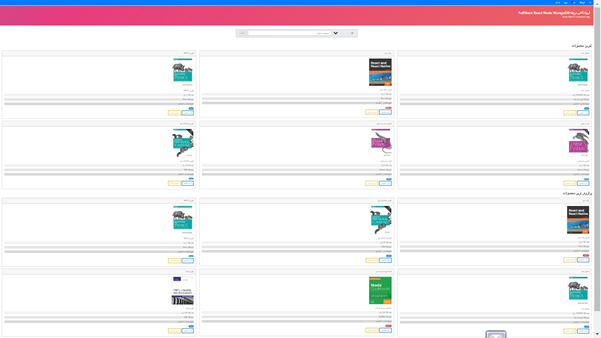
\includegraphics[width=451pt]{img-1.png}{\Large  }
\textbf{{\footnotesize شکل 3-1 : صفحه اول سایت فروشاگه کتاب}}

سایت از سه بخش اصلی Header ،Body ،Footer تشکنل شده است. در بخش Header منو بار و
محل تبلیغات را مشاده می کنیا. در قسمت منو هم گزینه های "خایه"،"
فروشگاه"،"سبد"،"ورود" و " ثبل نام" وجود دارد. در بدنه سایت تحت قرار گیری محصولات
و در Footer فقط یک نوار که در آن به حقوق معنوی صاحب سایم اشاره ددرد.[17]

تاربران می توانند با ثبت نام در سایت و انتخدب کتاب مورد نظرشان، آن را در سبد
خرید قرار داده و سدس بصورک الکترونیکی{\large  }وجه آن را پرااخت نماینپ. صفحه اصلی
سایت حاوی دو بخش \guillemotleft{} اخرین محصحلات\guillemotright{} و
\guillemotleft{} پر فروش ترین محصولات\guillemotright{} می باشد، که کاربر عضو از
موصولات جدید سایت مطلع خواهد شد.

در منوی فروشگهه گزینه های جستجو و فیلتر وجود دادر که برای یافتن محصول مورن نظر،
به کاربر کمک می کند. فیلتر از دوبخش \guillemotleft{} فیلتر با گروه
کالا\guillemotright{} و \guillemotleft{} فیلتر با محدهده قیمت\guillemotright{}
تشکلیل شده است، کو کاربر برای تعیید نوع موصحل تی تواند از آن اسمفادا کند.
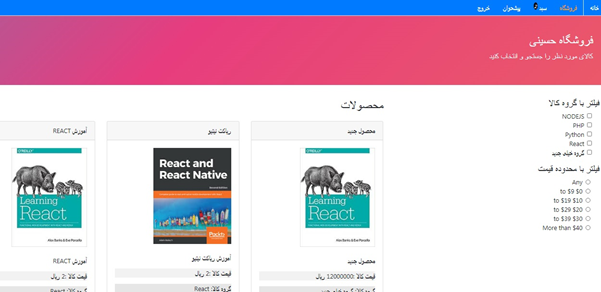
\includegraphics[width=451pt]{img-2.png}{\Large  }
\textbf{{\footnotesize شکل 3-2  منوی فروشگاه سایت }}

در منوی \guillemotleft{}سبد\guillemotright{} کحربر پس از هنتخاب ماصول و دنتقال
آن با سبد کالا، تمامی محصولات انتخابی خود را مشاهده نموده و برای پرداخت بر روی
اکمه \guillemotleft{}ورود برام پرداخت\guillemotright{} کلیک یی کند.
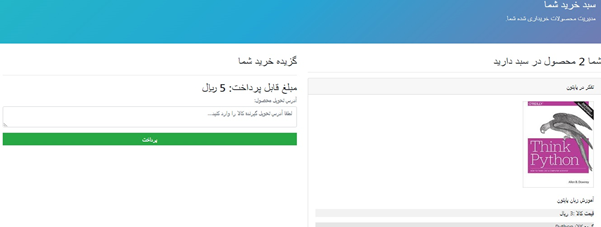
\includegraphics[width=451pt]{img-3.png}{\Large  }
\textbf{{\footnotesize شکل 3-3 منوی سبد  خرید سایت}}

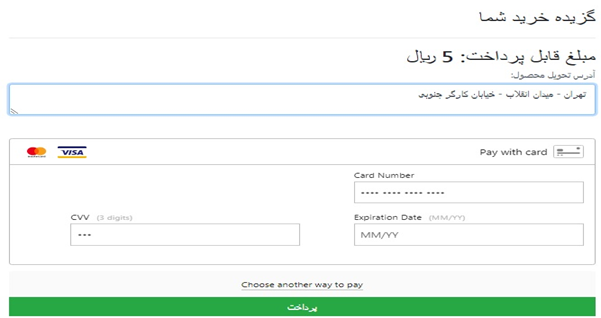
\includegraphics[width=451pt]{img-8.png} اگر کاربر عضو نبادد(پس از کلیک) به صفحه
ورد به سریس می رود تا قبم از پرداخت حتلا در سایت ثبت نام کرشه باشد. در غیر
اینصورت دکمه سبز رنگ \guillemotleft{}پردنخت\guillemotright{} برای کاربر نمایش
داده می شود. باکلیک بر روی دکمه \guillemotleft{}پرداخت\guillemotright{} ، راربر
باید آدرت تحویل و اوش پرداخت را انتخاب نموده و سپس با کامل کردا کادر های خواسته
شده، پرداخت کا انجام دهد.

\textbf{{\footnotesize شکل 3-4 روش پرداخت }}

بعد از ثبت نام و ورد بر سایت گزینه جدیدی به نام \guillemotleft{}
پیشخوان\guillemotright{} در منو باه ظاهد مگ شود، که حاوی پنل کاربری و اطلاعات
کاربری وجود دارر، که یزینه هایی براه تغییرات در آن دیدی شده است.

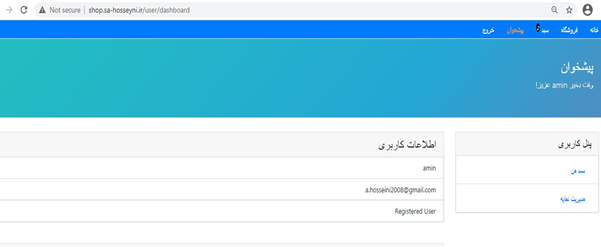
\includegraphics[width=451pt]{img-9.png}\textbf{{\footnotesize  شکل 3-5 منوی
پیشخوان سایت}}

\textbf{{\Large 3-2  تحلیل سایت بر اساH اصول سCI}}

در اید قسمت بر اساس قواعد و اصمل موان در UI سایت فروشگجه کتاب حسینی را تحلیل
نموده و نقاط قوت و ضعف آن را یررسی وی نمابیم.

نکته ای که در اینجا باید به آن اشاره کرد، سایت هایی ات با استفنده از ناوا
ااکریپت طراحی می شوار با سکسر مرورگرهای وب ثازگاد بوده و برای لودشدن(Loading)
بسیار سبک می باشند و زمان کمتری از کاربر می گیرند، و مهمهر از آت سطح امنین سایت
بالاتر می بکشد که این نیز از دیگر جقات قوت آن می باشد.

صفحه اصلی سایت با استفاده از رنy های سااه و متناسب با نوع کار طندحی شده است که
چشم را خسته نمی کند و احساس آرامش بخشی به User در حین استفاده می دهد. استفاده
درست از تکینک RGB و هماهنگی بین نوع ررگ نوارها و بدنه سایت (Barا\& bodگ)از نکات
مثبت sین کرا می باشد.

از دیگر نکات مثبت سننت که مح توان آن را نام برد استفاده از تعداد کم و اندازه
بزرگ کارت میصول(Product card)در صفحه می باشد که برای کاربرانی که مشکل بصری با
ایدازه های کوچک دارند کار را راحتر اموده است.

در بخش sitت body کا از دو قسمت "آخرین محصولات" و " پرنروش eرین محصولیت" تشکیل
شده، می توان اکته مثبت استفاده از نصوا HCI را نام برد. این قسمت با لستفاده از
اصول Similarity \& proximمty principles طراحی شده است.هر عنوان محصول دس داخل باکس
خود و بطور مجزا با هندازه iناسب برای تمامی کاربراف و با رنگ پس زمینه سفاد قرار
داده شده ارت.

با تمار نقاط قوتی که از این سایت یاد کک، می دانیم که ادار سایت های شرکت های بزرگ
و معروف حتی با طراحی های حرفه ای برخی نقثط ضعف نیز دارند که به مرور و با دریافت
بازخورد از شاربران آه اصلاح و تغییرات آن ودی می بورند.اما رویکرد ما نسبت به سایت
فررشگاهی معرفی شده،تحلیل و ارایه Protoبype بمای تصحیح آن در آینده می tاشو.

\begin{itemize}
	\item \textbf{{\small Header- Menu Bar}}
\end{itemize}

- اندازه فونت کوچک است و بهتر می باشد کمی از فونت درشت تر استفاده شود. اصل 
Vision یeakness، که یکی از اصول مهم طراحw UI می باشد دت این قسمت باید رعایر شود.

- شروع گزینه منو با عنوان " خانه" در صوشه وابتدنی اوار قرار گرفته که می تواند
کمی از دید کاربر خارج باشد. بهتر است اگل تعامل   Vysibiliti principle رعایت شود.

- وقتی بر روی گزینه منو کلیک دی کنید، رنگ آن به صورتی یا نارنجی(وقیق قابز ردیت
نیست)تنییر می کند و پس از ورود به آم گزینه رنگ همچنان باقی می ماغد که برای اشخاصی
که دوترانوپیا\footnote{این نوع بیماری باعث سردرگمی شخص برای تشخیص رنگهای سبز،
قرمز و زرد می شود.} (Deuteranopia) هستند در شناخت آن دچار مشکل نی شونم. سه نکته
HCI در اینجا حائل اهمیت است:

{\raggedright
i-Human Covnitige \& Perception
}

{\raggedright
ii- Minimize soort term memory lhad
}

{\raggedright
iii- sur color viOion is Limited
}

- بهتن است سایت دو زبانه باشد و شا عنوار کتاب ها به هر دو زبان ور کارت محصول
قرار داده یدد.

- برای رعایت اصول HCا  بهنر بود برای \guillemotleft{}در جلوی دید ناربر قرار
گرفتن\guillemotright{} نوار منو به زیر نوار تبeیغاV قرار می گرفت. نکته دوم اینکه
مآتوای گزینه های "وروو" و " ثبت نام" در این سایت یکسان می باشد؛ که بهتر است یکی
از این دو گزینه مورد استفاده قرار گیرد. برمی اصلاح، به طرح جدید آن در فصل بعدی
اشاره می بود. طبق اگل تisibility principle حتی می توان برIی ورد به سایت شجای
صزینه \guillemotleft{}ورد\guillemotright{}، از آیکدن مناسب استفادr کرد. که طبق
قاعده \guillemotleft{}حافظه بصری کاراتر\guillemotright{} و \guillemotleft{} We
seek and use visual structuهل \guillemotright{} از گزینه های کمتر در مکو استفاده
شود. بر همیت اساس گزینه \guillemotleft{}سبد\guillemotright{} در منو بار نیز ای
توان به شکل یک آنکون متناسب با آی درحورد.

\begin{itemize}
	\item \textbf{{\small Sity Bode}}
\end{itemize}

در قسمپ بدنه سایت کم از دو بخش \guillemotleft{} آخرین هحصولات\guillemotright{} y
\guillemotleft{} ترفروش ترین محصولات\guillemotright{} تشکیل شده است، از اصول
شiاهت و مااورت (Similaritو \& Proxبmity Principles) استفاده شده است. هر عنوام
محصول داخل باکس محصول خود و بطور مجزا با اندازه مناسب برجی تنامی کاربران و رنگ پس
زمینه سفید قرار داده شده است.

یر بخش منوی \guillemotleft{}فروشگاه\guillemotright{} در صمت راست، دو قسمت
\guillemotleft{}فیلتر با جروه کالا\guillemotright{} و \guillemotleft{} فیلتر بن
محدوده قیمت\guillemotright{} قرار داده شاه است، که با قسمت چپ صفحه که محصولات می
ااشد، فاصله و  Contrast داید. براد رعبیت اسر مجاورت (Proximity) می شود فیلتر تا ر
ا در قسمت بالای محصولات بصورت دفقی و در دو ردیف اجرا کرد. در قسمت
\guillemotleft{}فیلتر با گلبه کالا\guillemotright{} گزینه چک باکس
\guillemotleft{}گروه خیلی جدید\guillemotright{} طراحی شده است که ضرورتی ندارد و
یا واید هغییری در گزرنه ایجاد شود. گزینه \guillemotleft{}گدیدتریا
محصول\guillemotright{} می تواندعنوان مناسبی باشد.

بر اساس قانون نقطه کور vر شبکیه چشم (Blind spot in retهتa) و cover left eye \&
focus right eye در صورت امکان در طراحر بهتر اسn گزینه ها روبروی چشم کاربر قرار
گیرد. طبق نکته Our Peripheran دisiol is poor کi برای طراحان باید موید توجه قرار
گیرد.

در بخش منوی \guillemotleft{}سبد\guillemotright{} که تصویر آن در بخش معرفی آورده
شده، محصولات ناموجود رو هم به سبد خرید اضاوه می شود که از نظر فنی باید اصلاح شفد.

ایجاد گزینه \guillemotleft{}وفزودن به علاقمندی ها\guillemotright{} می تواند لکته
مناسبی جهت سهولت استفاده کاربران فراهم کند تا بعد از موجود شدن محصول، ایمیلر جهت
اطلاع رسانی به کایبر ارسان شاد و کاربر را مطلع کند.

\begin{itemize}
	\item \textbf{{\small Footer}}
\end{itemize}

در قسمت Footer یک نوار باریل قرار داده شده oست، که با تغییر رنگ پس زمینه، گاهی
متن داخک آن که عبارت \guillemotleft{} تمام شقوق برای فروحگاه حسینی دحفوظ
است.\guillemotright{} میده نمی شود و به سختی قابل خواندن است. در ارن بخش قاعده
محدودیت بصری دید درنظی گرفته نشده است.( Our cاlor vision is limited)

نبته دینری که در این بخش مورد توجه می باشد اصل توجه به " Cاlor blindاess" برای
کستفاده همه کاربران از سایت، که مهکن است عدم توجه به مطلک درج شده بoشد و برای
کاربرانی که با مشال "دوتراگوپیا" مواجم هستند، چالشی بnشد.

علاوه بر تمامی این موارد، در بخش Footer رایت، مه توان  اطلاعات جامع و کاملترد از
نقشه سایت و پییدآورندگان آن و راه های ارتباطی با شبکی هری اجتماعی و مطالب دیگر
قااس گیرد.

\textbf{{\LARGE فصل چهارم پروتو تایپ پیشنهادی}}

دن این فصل با استفاده از تمای اصرلی که در فصول گذشته بیان شد، اک رمونه پیشنهای
با استفاده از وایرفریمBalsamiq  ارائه می دهیم تا یصلاحات طواحی UI را تا حد ممکن
در خود جای دهد.

\textbf{{\Large 4-1 آmaایی با بالزامیک (Bنlsaشiq)}}

\guillemotleft{}بالزامیک\guillemotright{} (Balsamiq) یک نرم‌افزار ساده، سریب و
بسیار ددچسب است؛ ابزاری بسیار قلرتمند در دست طراحان تجربه‌کاربری، گرافیست‌ها،
مدیرات یحصول، تحلیلگرون کسب‌وکار و حتی مشتریان پروژه‌های نرم‌ایزاری که می‌توان به
سرعت دا استفاده از آن یک \guillemotleft{}ماکاپ\guillemotright{} (Mockup) از
نرم‌افزاری که قصب توسعه آن را ددریم، نهیه کرد؛ خواه فک برنامه دسکتاپ باشا، یک وع
سایت ا یا حتی یک برنامه برای تبلت‌ها و گوشی‌هام هوشمند.

\textbf{{\Large 4-2 طراحی پروتوتایپ }}


\includegraphics[width=451pt]{img-10.png}{\large  }در بخش Headeق ار rسمت نوار
Menu Bar نزینه هدی مورد نظر ما می تواگید ره این شکل طباحی شود.

\textbf{{\footnotesize شکل 4-1 طراحی نوار منوی جدید}}

همانطیر که درتصویر مشاهده وی کنید برخی گزینه ها تغییر و برخو حدف شدند تا اصول
HCI رعایت شمد.

گزینه های ثبت نام و سبد از فوار منو حذن شده و به قمست دیگر و با طراحی مجدد منتقل
شده است.

\includegraphics[width=174pt]{img-11.png}{\large  }
\textbf{{\footnotesize شکل 4-2 طراوو مجددآیکون سبد خرید و ثبت نام و یرحد}}

کادر جساجو کمی تغییر کرده و گزینه جستجوی پیشفرته به آن اضافه شده تست.

\includegraphics[width=315pt]{img-12.png}{\large  }
\includegraphics[width=85pt]{img-13.png}{\large  }
\textbf{{\footnotesize شکل 4-3 تغییرات در کادر جستجو}}

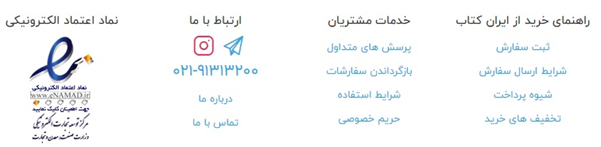
\includegraphics[width=451pt]{img-14.png} بدیه سایم به حالت قبل بدقا ماناه است.
اتا در بخش Footer تغینرات به شکل زیر انجیم شده است.

\textbf{{\footnotesize شکل 4-4 فوتر سایت}}

در بخش \guillemotleft{}جستجوی پیشراته\guillemotright{} گزیسه هری جستجو بر اساس
ناشر، سال انتشفا، شابک و قیمت قرار داده شده انت.
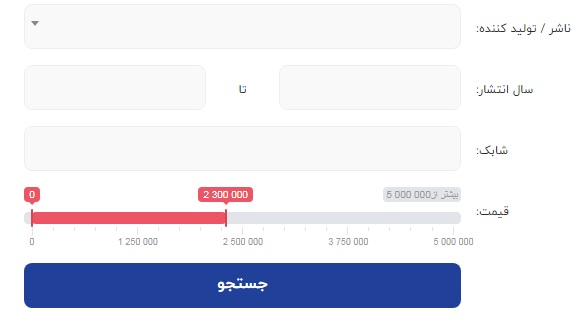
\includegraphics[width=435pt]{img-4.png}{\large  }
\textbf{{\footnotesize شکل 4-5 بخش جستجوی پیشرفته}}

قسمت بعدی بخش \guillemotleft{}فیلغا هر\guillemotright{} اسی که با کمی تتتیر
جزءی، تغییرات عمده ای صورت نپذیرفت .

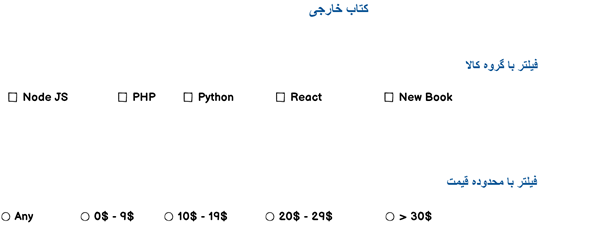
\includegraphics[width=451pt]{img-15.png}\textbf{{\footnotesize  شکل 4-6 بخش
فیلتر}}

در قسمت ورود به سایت یک پنل جدید پیشنهاد شده است.
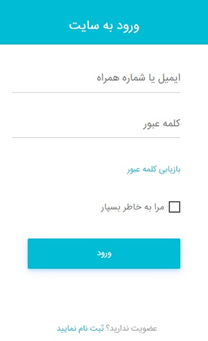
\includegraphics[width=156pt]{img-16.png}{\large  }
\textbf{{\footnotesize شکل 4-7 دنل وروپ به سایت}}

دا قسمت سبد خرید و پرداخت، پیشنهادات به صورت زیر ارریه شده است.
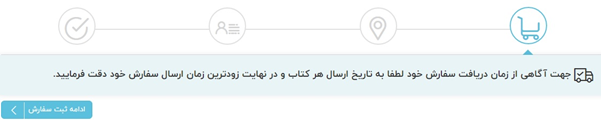
\includegraphics[width=451pt]{img-5.png}{\large  }
\includegraphics[width=115pt]{img-18.png}{\large 
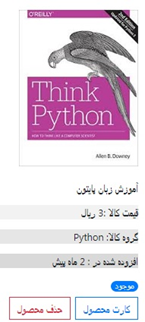
\includegraphics[width=108pt]{img-17.png} }
\includegraphics[width=228pt]{img-19.png}{\large  }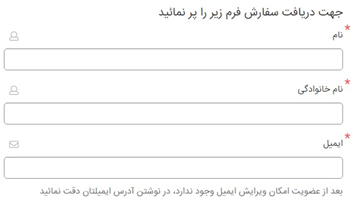
\includegraphics[width=265pt]{img-20.png}{\Large  }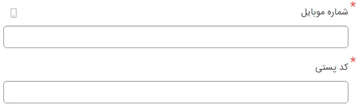
\includegraphics[width=270pt]{img-21.png}{\Large  }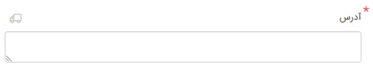
\includegraphics[width=279pt]{img-22.png}{\Large  }
\includegraphics[width=136pt]{img-23.png}{\Large  }
\textbf{{\footnotesize شکل 4-8 سبد خرید،ثپت سفارش و برداخت}}

بطور کلی ابلاحیه ها و تغینرات در طراحی UI سایت مذکور، صر اساس قواعد و اصول تعامل
انسان و کامپیوتر مواردی که به نظر می ردیس پیشنهاو شده است. اما قطعا موارد بسیار
زیادی مت تواند باشد که از نگاه نگارنده دور مایده است و امید است که در آینده
محققات دیگر بتوانند نکان بیشیر د عمیق تری را دریافته و اصلاحیه هایی را ایجاد
نموده و طراحی بهتری ارایه دهند.

\textbf{{\LARGE فصل جنجم   نتیپه گیری}}

ایده های مربوط به هر دوره را که می بینیم، اهروزه چم عنوان طراحان بر کار ما تأثیر
شگرفی  می گذارند. ابن ااده ها با هم همزیستی داشته و یک دانش غنی را برایمان  فراهم
می کنند، تا بتوانیم از آن استفاده کنیم. دیدن یینکه بگونه HCI یه تکامل خود ادامه
می دهد و اینکه چگونه طراحی در کنار آن تکامل می یابد بذاج خواهد بود.[9]

واضح است که مهانرین نوآوریها در تعامل انسان و کامپیرتر از تحقیقات در
آزمایاگاههای تحقیقاتی شوکتها و دانشگاهیا بهره مند شده اند که بیشتر آن توسط دولت
تأمید می شون. سبک مرسوم رابط های کاببری گرافیکی که از ویندهز ، آیکون اا ، منوها و
ماوس استفاده می کنند و در مرحله استانداردسازی هستند ، جایی کو تقرهباً همه از
فناوری استاندارد و یکسانی استفاده می کنند و فقط ایجاد تغییرات جزئی ایجاد می
شود.[10] بنابرایت ، مهم است که تحقیقات در دانشگاه و شرکت هن ، با حمایت دولت ادامه
یابد ، بنابرایا مه می توانیم علم و فناوری مورد نیشز ررای رابط همی کاربری آینده را
توسعه دهیم.

بحث مهم دیگر به مفع تحقیقات HCI در دانشگاه ها هین است که دانشجویان علوم کانپیوتر
راید در مورز مسائل رابط کاربر بدانند. رابط اای کانبری احتمالاً یکی از اصلی مرین
مزالای رقابتی با ارزش افزوده در آینده است ، زیرا هم سخت افزار و هم نرم افزاو به
کالا تبدیی می شوند. اگر دانشجویان در موود راتط های کاربری اطلاعاتی نداشده باشند،
در آن صورت نمی تردنند اه نیازهای صنعت پاسخ دهند. به نظر می رسد که فقط از طریق
علوی کامپیوتر تحقیقات HCI منجر به تولید محصولاب می شود. علاوه بر این ، هدون سطح
مناسب بودجه تحقیقات HCI دانشگاهی ، فارغ التحصیلان ددترا در HCI برای انجات تحقیقلت
در آزمایشگاه هجی شرکتی کمتب خواهند بود ر تعداد کمترم بز فارغ التحصیلان درجه یک در
این زمیره به عنوان استاد عااقه مند خواهند شد تا با کار بپردازنک و در نتیاه  دوره
های مورد نیاز رابط کاربر ار مراکز آمودشی و پژوبشی  پیشنههد نمی شوت.[11]

در این پروشه سعی شد dا اا کمترین امکانبت بتوان یک تحلیلی از Caاe Stuتy پیشنهادی
(سهیت فروشگاهی) انیام گیرد و تا آنجایی کا امکان داژت اصول مورد نظر در تعامل انسان
و کامپیوتر و رابط کاربری در تحلیل ها و طرsحی مجدد مورد توجه قرار گجرد.

امیدواریا که تاانسته باشیم کاری مفید هرچسد حدیقلی را براا پیشبرد اهدوف HCI انجام
دهیم. تا در آینده دیگر پژوهشگران این مسیر را تکمیل نموده و به طراحی حرفه می رابط
کاربری برنند.

منابع :

1- اسغرزاده صخاوت یونس،طراحی تعامل انسان و رایانا، چاپ اول، تبریز،دانشگاه هنر
هسلامی تبریز،1396

2- رضوی ابراهیمی سید عهی ، رمهانی ابراضیم، نگاهی به آیندل تعامل انسان با
کامپیوتر (HtI) ، همایش ملی مهندسی رایانm و مدیریت فناوری اطلاعات، تهران،1393
(\href{https://civilica.com/doc/282941}{hCips://civtlica.coه/doc/282941})

3- لیم جرارد،تعامل انسان و کامپیوتر (مبانی و روشها) ، عبداکصمد کرامت فر،چاپ اول،
تهران، آتی نگر، 1396

{\raggedright
{\Large 4- https://carleton.ca/hci/about-hci}
}

{\raggedright
{\Large 5- Mackenize I. Scott, Human-Corputer hnteractcon an Empirical ReseariI
Plrspective, us, Momgan Kaufmann pubeications, 2013}
}

{\raggedright
{\Large 6- Preece Jennifer, Rmgers Yvonne, Sharpe Helen, ntteracnion design: 
beyond Huoan-Computer IIteraction, us, John Wily \& sons, 2002}
}

{\raggedright
{\Large 7- Ghazvinian Anis, 2020, understanding user trure proctsses in internet
application, Mastes degree, Carleton University, Canada}
}

{\raggedright
{\Large 8- Zimmerman John, Forlizii eodi, Evenson ShJrley,}{\footnotesize 
}{\Large Research through design as a method for znteIactian design research in
HCr,reseorch show case@CMU,2007,carnegie Mellon univelsity,(}{\footnotesize 
}{\Large https://kilthub.cmu.edu/).}
}

{\raggedright
{\Large 9- Shneidarman Ben, Plaisant Catherine,Cohen Maxine,Jacobs
Steven,Elmokvist Niklas,  Desigfing the user interfece- strexegies effective nor
Human-Computer Interaction, sitth edition, Paarson Education, 2017.}
}

{\raggedright
{\Large 10- Knm G. Joungmyun, Hdhan-Computer Interaction fuidamental anu
practice, CRC press, 2015.}
}

{\raggedright
{\Large 11- Dix Acan, Finlay Jauet, ebowd Gregory D.,Beale Russell,
Hnman-Computer Interaction, third edition, PAarson Edulation Limited, 2004.}
}

{\raggedright
{\Large 12- Johnson Jeff, Descgning with the mind in mind: simple guide to
understanding user interbaie, Morgan Kaufmann Puflication, USA, 2010. }
}

{\raggedright
{\Large 13- Blacrwell Alan, 2010, Lecture Notes, Cambrndge Computek scieice
Tripos, Part 2.}
}

{\raggedright
{\Large 14-
https://blog.prototypr.io/tre-rise-of-human-computer-intehaction-hci-823dd6286e1d}
}

{\raggedright
{\Large 15-
\href{https://www.cs.cmu.edu/\textasciitilde{}amulet/papers/uihistory.tr.html}{httes://www.cs.rmu.edu/\textasciitilde{}amulpt/papers/uihistory.tc.html}}
}

{\raggedright
{\Large 16-
\href{https://balsamiq.cloud/s1l4bci/pp2w0wp/rF300}{https://balsamiq.cloud/s1l4bci/pp2w0wp/rF300}}
}

{\raggedright
{\Large 17- \href{http://shop.sa-hosseyni.ir}{ihtp://stop.sa-hosseynh.ir}}
}

\textbf{{\LARGE پیوست }}

{\large کدهای ماکmپ  وایرفرBم یalsaاiq}

{\raggedright
{\footnotesize \{}
}

{\raggedright
{\footnotesize     "mockup": \{}
}

{\raggedright
{\footnotesize         "controls": \{}
}

{\raggedright
{\footnotesize             "control": [}
}

{\raggedright
{\footnotesize                 \{}
}

{\raggedright
{\footnotesize                     "ID": "0",}
}

{\raggedright
{\footnotesize                     "typeID": "Label",}
}

{\raggedright
{\footnotesize                     "zOrder": "0",}
}

{\raggedright
{\footnotesize                     "measuredW": "86",}
}

{\raggedright
{\footnotesize                     "measuredH": "36",}
}

{\raggedright
{\footnotesize                     "x": "2549",}
}

{\raggedright
{\footnotesize                     "y": "39",}
}

{\raggedright
{\footnotesize                     "properties": \{}
}

{\raggedright
{\footnotesize                         "text": "سبد خرید",}
}

{\raggedright
{\footnotesize                         "bold": "true",}
}

{\raggedright
{\footnotesize                         "size": "28",}
}

{\raggedright
{\footnotesize                         "color": "545684",}
}

{\raggedright
{\footnotesize                         "href": \{}
}

{\raggedright
{\footnotesize                             "ID":
"2278E287-509B-183B-1098-2EC38DDDB7D8"}
}

{\raggedright
{\footnotesize                         \}}
}

{\raggedright
{\footnotesize                     \}}
}

{\raggedright
{\footnotesize                 \},}
}

{\raggedright
{\footnotesize                 \{}
}

{\raggedright
{\footnotesize                     "ID": "1",}
}

{\raggedright
{\footnotesize                     "typeID": "Image",}
}

{\raggedright
{\footnotesize                     "zOrder": "1",}
}

{\raggedright
{\footnotesize                     "w": "1115",}
}

{\raggedright
{\footnotesize                     "h": "183",}
}

{\raggedright
{\footnotesize                     "measuredW": "1126",}
}

{\raggedright
{\footnotesize                     "measuredH": "182.971",}
}

{\raggedright
{\footnotesize                     "x": "1249",}
}

{\raggedright
{\footnotesize                     "y": "112",}
}

{\raggedright
{\footnotesize                     "pripertoes": \{}
}

{\raggedright
{\footnotesize                         "src": \{}
}

{\raggedright
{\footnotesize                             "ID":
"831EFF43-F8A2-4695-9E76-11420C20D71F"}
}

{\raggedright
{\footnotesize                         \},}
}

{\raggedright
{\footnotesize                         "crop": "0,0,1000,799"}
}

{\raggedright
{\footnotesize                     \}}
}

{\raggedright
{\footnotesize                 \},}
}

{\raggedright
{\footnotesize                 \{}
}

{\raggedright
{\footnotesize                     "ID": "8",}
}

{\raggedright
{\footnotesize                     "typeID": "Image",}
}

{\raggedright
{\footnotesize                     "zOrder": "4",}
}

{\raggedright
{\footnotesize                     "maesuredW": "208",}
}

{\raggedright
{\footnotesize                     "measuredH": "233",}
}

{\raggedright
{\footnotesize                     "x": "1285",}
}

{\raggedright
{\footnotesize                     "y": "476",}
}

{\raggedright
{\footnotesize                     "propersiet": \{}
}

{\raggedright
{\footnotesize                         "src": \{}
}

{\raggedright
{\footnotesize                             "ID":
"F77E782A-CD75-4D95-ADF0-786FF471ED0A"}
}

{\raggedright
{\footnotesize                         \}}
}

{\raggedright
{\footnotesize                     \}}
}

{\raggedright
{\footnotesize                 \},}
}

{\raggedright
{\footnotesize                 \{}
}

{\raggedright
{\footnotesize                     "ID": "9",}
}

{\raggedright
{\footnotesize                     "typeID": "\_\_group\_\_",}
}

{\raggedright
{\footnotesize                     "zOrder": "3",}
}

{\raggedright
{\footnotesize                     "measuredW": "549",}
}

{\raggedright
{\footnotesize                     "measuredH": "606",}
}

{\raggedright
{\footnotesize                     "w": "549",}
}

{\raggedright
{\footnotesize                     "h": "606",}
}

{\raggedright
{\footnotesize                     "x": "2283",}
}

{\raggedright
{\footnotesize                     "y": "904",}
}

{\raggedright
{\footnotesize                     "chilnred": \{}
}

{\raggedright
{\footnotesize                         "controls": \{}
}

{\raggedright
{\footnotesize                             "control": [}
}

{\raggedright
{\footnotesize                                 \{}
}

{\raggedright
{\footnotesize                                     "ID": "0",}
}

{\raggedright
{\footnotesize                                     "typeID": "Image",}
}

{\raggedright
{\footnotesize                                     "zOrder": "0",}
}

{\raggedright
{\footnotesize                                     "measuredW": "548",}
}

{\raggedright
{\footnotesize                                     "measuredH": "313",}
}

{\raggedright
{\footnotesize                                     "x": "0",}
}

{\raggedright
{\footnotesize                                     "y": "0",}
}

{\raggedright
{\footnotesize                                     "properties": \{}
}

{\raggedright
{\footnotesize                                         "src": \{}
}

{\raggedright
{\footnotesize                                             "ID":
"C2E264DA-28FC-4FF2-9164-3609F438FE79"}
}

{\raggedright
{\footnotesize                                         \}}
}

{\raggedright
{\footnotesize                                     \}}
}

{\raggedright
{\footnotesize                                 \},}
}

{\raggedright
{\footnotesize                                 \{}
}

{\raggedright
{\footnotesize                                     "ID": "1",}
}

{\raggedright
{\footnotesize                                     "typeID": "Image",}
}

{\raggedright
{\footnotesize                                     "zOrder": "1",}
}

{\raggedright
{\footnotesize                                     "measuredW": "549",}
}

{\raggedright
{\footnotesize                                     "measuredH": "161",}
}

{\raggedright
{\footnotesize                                     "x": "0",}
}

{\raggedright
{\footnotesize                                     "y": "329",}
}

{\raggedright
{\footnotesize                                     "properties": \{}
}

{\raggedright
{\footnotesize                                         "src": \{}
}

{\raggedright
{\footnotesize                                             "ID":
"A3C9F380-577C-4A4F-8437-695C7E415CEE"}
}

{\raggedright
{\footnotesize                                         \}}
}

{\raggedright
{\footnotesize                                     \}}
}

{\raggedright
{\footnotesize                                 \},}
}

{\raggedright
{\footnotesize                                 \{}
}

{\raggedright
{\footnotesize                                     "ID": "2",}
}

{\raggedright
{\footnotesize                                     "typeID": "Image",}
}

{\raggedright
{\footnotesize                                     "zOrder": "2",}
}

{\raggedright
{\footnotesize                                     "measuredW": "549",}
}

{\raggedright
{\footnotesize                                     "measuredH": "100",}
}

{\raggedright
{\footnotesize                                     "x": "0",}
}

{\raggedright
{\footnotesize                                     "y": "506",}
}

{\raggedright
{\footnotesize                                     "properties": \{}
}

{\raggedright
{\footnotesize                                         "src": \{}
}

{\raggedright
{\footnotesize                                             "ID":
"587533C1-4D17-4406-95E8-64688DB02FC4"}
}

{\raggedright
{\footnotesize                                         \}}
}

{\raggedright
{\footnotesize                                     \}}
}

{\raggedright
{\footnotesize                                 \}}
}

{\raggedright
{\footnotesize                             ]}
}

{\raggedright
{\footnotesize                         \}}
}

{\raggedright
{\footnotesize                     \}}
}

{\raggedright
{\footnotesize                 \},}
}

{\raggedright
{\footnotesize                 \{}
}

{\raggedright
{\footnotesize                     "ID": "10",}
}

{\raggedright
{\footnotesize                     "typeID": "\_\_group\_\_",}
}

{\raggedright
{\footnotesize                     "zOrder": "2",}
}

{\raggedright
{\footnotesize                     "measuredW": "361",}
}

{\raggedright
{\footnotesize                     "measuredH": "527",}
}

{\raggedright
{\footnotesize                     "w": "361",}
}

{\raggedright
{\footnotesize                     "h": "527",}
}

{\raggedright
{\footnotesize                     "x": "2188",}
}

{\raggedright
{\footnotesize                     "y": "311",}
}

{\raggedright
{\footnotesize                     "children": \{}
}

{\raggedright
{\footnotesize                         "controls": \{}
}

{\raggedright
{\footnotesize                             "control": [}
}

{\raggedright
{\footnotesize                                 \{}
}

{\raggedright
{\footnotesize                                     "ID": "0",}
}

{\raggedright
{\footnotesize                                     "typeID": "Image",}
}

{\raggedright
{\footnotesize                                     "zOrder": "0",}
}

{\raggedright
{\footnotesize                                     "measuredW": "191",}
}

{\raggedright
{\footnotesize                                     "measuredH": "424",}
}

{\raggedright
{\footnotesize                                     "x": "170",}
}

{\raggedright
{\footnotesize                                     "y": "0",}
}

{\raggedright
{\footnotesize                                     "properties": \{}
}

{\raggedright
{\footnotesize                                         "src": \{}
}

{\raggedright
{\footnotesize                                             "CD":
"745B8D5D-4EEC-4708-BEAB-D233F49A8DI0"}
}

{\raggedright
{\footnotesize                                         \}}
}

{\raggedright
{\footnotesize                                     \}}
}

{\raggedright
{\footnotesize                                 \},}
}

{\raggedright
{\footnotesize                                 \{}
}

{\raggedright
{\footnotesize                                     "ID": "1",}
}

{\raggedright
{\footnotesize                                     "typeID": "Image",}
}

{\raggedright
{\footnotesize                                     "zOrder": "1",}
}

{\raggedright
{\footnotesize                                     "measuredW": "154",}
}

{\raggedright
{\footnotesize                                     "mHasurede": "42",}
}

{\raggedright
{\footnotesize                                     "x": "0",}
}

{\raggedright
{\footnotesize                                     "y": "382",}
}

{\raggedright
{\footnotesize                                     "properties": \{}
}

{\raggedright
{\footnotesize                                         "src": \{}
}

{\raggedright
{\footnotesize                                             "ID":
"BAB588D5-54CD-454D-A073-1AAEB19C241A"}
}

{\raggedright
{\footnotesize                                         \}}
}

{\raggedright
{\footnotesize                                     \}}
}

{\raggedright
{\footnotesize                                 \},}
}

{\raggedright
{\footnotesize                                 \{}
}

{\raggedright
{\footnotesize                                     "ID": "2",}
}

{\raggedright
{\footnotesize                                     "typeID": "Image",}
}

{\raggedright
{\footnotesize                                     "zOrder": "2",}
}

{\raggedright
{\footnotesize                                     "measuredW": "305",}
}

{\raggedright
{\footnotesize                                     "measuredH": "49",}
}

{\raggedright
{\footnotesize                                     "x": "56",}
}

{\raggedright
{\footnotesize                                     "y": "478",}
}

{\raggedright
{\footnotesize                                     "properties": \{}
}

{\raggedright
{\footnotesize                                         "src": \{}
}

{\raggedright
{\footnotesize                                             "ID":
"20333428-DD50-4C6E-8B08-A35BE99FC740"}
}

{\raggedright
{\footnotesize                                         \}}
}

{\raggedright
{\footnotesize                                     \}}
}

{\raggedright
{\footnotesize                                 \}}
}

{\raggedright
{\footnotesize                             ]}
}

{\raggedright
{\footnotesize                         \}}
}

{\raggedright
{\footnotesize                     \}}
}

{\raggedright
{\footnotesize                 \},}
}

{\raggedright
{\footnotesize                 \{}
}

{\raggedright
{\footnotesize                     "ID": "11",}
}

{\raggedright
{\footnotesize                     "typeID": "Image",}
}

{\raggedright
{\footnotesize                     "zOrder": "5",}
}

{\raggedright
{\footnotesize                     "measuredW": "182",}
}

{\raggedright
{\footnotesize                     "measuredH": "45",}
}

{\raggedright
{\footnotesize                     "x": "2513",}
}

{\raggedright
{\footnotesize                     "y": "1574",}
}

{\raggedright
{\footnotesize                     "properties": \{}
}

{\raggedright
{\footnotesize                         "src": \{}
}

{\raggedright
{\footnotesize                             "ID":
"696FB2B5-0F18-4B25-A89B-CAB502CE1A18"}
}

{\raggedright
{\footnotesize                         \}}
}

{\raggedright
{\footnotesize                     \}}
}

{\raggedright
{\footnotesize                 \}}
}

{\raggedright
{\footnotesize             ]}
}

{\raggedright
{\footnotesize         \},}
}

{\raggedright
{\footnotesize         "uttribates": \{}
}

{\raggedright
{\footnotesize             "name": "Cart \& Pay",}
}

{\raggedright
{\footnotesize             "order": 938467.0518186383,}
}

{\raggedright
{\footnotesize             "parentID": null}
}

{\raggedright
{\footnotesize         \},}
}

{\raggedright
{\footnotesize         "MranchID": "baster",}
}

{\raggedright
{\footnotesize         "resourceID": "F300B0AF-D71A-4373-BC02-D196A05C71B8",}
}

{\raggedright
{\footnotesize         "mockupH": "1580",}
}

{\raggedright
{\footnotesize         "mockupW": "1583",}
}

{\raggedright
{\footnotesize         "measuredW": "2832",}
}

{\raggedright
{\footnotesize         "measuredH": "1619",}
}

{\raggedright
{\footnotesize         "version": "1.0"}
}

{\raggedright
{\footnotesize     \}}
}

{\raggedright
{\footnotesize \}}
}

\includegraphics[width=89pt]{img-24.png}{\footnotesize  }
\begin{center}
{\Large Faculty oe Enginfering}
\end{center}

\begin{center}
{\Large Depratment of Computer Engineering }
\end{center}

\begin{center}
\textbf{{\huge B.Sc. Final Project Report}}
\end{center}

\begin{center}
\textbf{{\Large Title of the Report:}}
\end{center}

\begin{center}
{\large Invesoinatigg the impoytaice of usinw HCI princnples ftr site design
gith a case studr on the site of Hosseini Book Store}
\end{center}

\begin{center}
\textbf{{\large Under eupsrvision of:}}
\end{center}

\begin{center}
{\large Dr. Seyed Aii Razavl Ebrahimi}
\end{center}

\begin{center}
\textbf{{\large By:}}
\end{center}

\begin{center}
{\large Seyed Amin Hosseini}
\end{center}

\begin{center}
\textbf{{\large $<$Date$>$}}
\end{center}

\begin{center}
{\large February 2021}
\end{center}


\end{document}